\documentclass[english,11pt,a4paper]{article}
\usepackage[T1]{fontenc} % --------------| More characters.
\usepackage[utf8]{inputenc} % ---------| Direct use of scandinavian letters.
\usepackage{float} % --------------------| More options for floats.
\usepackage{graphicx} % -----------------| Support more image formats.
\usepackage{booktabs} % -----------------| Better-looking tables.
\usepackage{tabularx} % -----------------| Better tables
\usepackage{subfig} % -------------------| Subfigures.
\usepackage[a4paper]{geometry} % --------| Adjusting page margins.
\usepackage{amsmath,amssymb,amsfonts} % -| Various math, including eqref.
\usepackage{xcolor} % --------------------| Allows defn. of custom colors.
\usepackage{babel}
\usepackage{url}

% XY-pic. Used for creating illustrations.
\input xy
\xyoption{all}

% Styling captions.
\usepackage{caption}
\captionsetup{margin=10pt,font=small,labelfont=bf}

% Changing section header fonts.
\usepackage{sectsty}
\allsectionsfont{\normalfont\sffamily}

%******************************************************************************
% Includes the listings package and sets some settings for it.
% REQUIRES the `color' package.
%******************************************************************************

\usepackage{listings} % -----------------------| Used for source code listings.
\definecolor{lst-gray}{RGB}{100,100,100}  % ---|Color for line-numbers.
\definecolor{lst-light-gray}{RGB}{250,250,250} % Background color for listings.
\definecolor{lst-dark-green}{RGB}{45,111,0} % -| Dark green for comments.
\lstset{
  aboveskip=0em, % -------------------| Skip above listing box.
  backgroundcolor=\color{lst-light-gray}, % Background color.
  basicstyle=\ttfamily\scriptsize, % -| Default font style.
  belowskip=\topskip, % --------------| Skip below listing box.
  breakatwhitespace=false, % ---------| Automatic breaks only at whitespace?.
  breaklines=true, % -----------------| Sets automatic line breaking.
  captionpos=t, % --------------------| Sets the caption-position to bottom.
  commentstyle=\color{lst-dark-green}, % ------| Comment style.
  escapeinside={\%*}{*)}, % ----------| For adding LaTeX within code.
  frame=single, % --------------------| Adds a frame around the code.
  keepspaces=true, % -----------------| Keeps spaces in text.
  keywordstyle=\color{blue}, %--------| Keyword style.
  language={C}, % --------------------| The language of the code.
  literate={æ}{{\ae}}1 % -------------| Character conversions
           {Æ}{{\AE}}1
           {ø}{{\oe}}1
           {Ø}{{\OE}}1
           {å}{{\aa}}1
           {Å}{{\AA}}1
           {µ}{{\ensuremath{\mu}}}1,
  numbers=left, % --------------------| Line-number position: none/left/right.
  numbersep=5pt, % -------------------| Distance between line-numbers and code.
  numberstyle=\tiny\color{lst-gray}, %| The style that used for line-numbers.
  rulecolor=\color{black}, % ---------| Frame color.
  showspaces=false, % ----------------| Show spaces with underscores.
  showstringspaces=false, % ----------| Underline spaces within strings.
  showtabs=false, % ------------------| Show tabs with underscores.
  stepnumber=1, %---------------------| Step between two line-numbers..
  stringstyle=\color{red}, % ---------| String literal style.
  tabsize=4, % -----------------------| Sets default tabsize to 2 spaces.
  title=\lstname % -------------------| Show the filename of included file.
}
\usepackage{url}

\author{Dzenan Dumpor \\ Einar Baumann \\ Teodor Heggelund}
\title{TMA4280 Exercise 4}

\begin{document}
\maketitle

\clearpage
\section{Program} % (fold)
\label{sec:program}
The source for the program can be found on Github: \url{https://github.com/einar90/tma4280_gruppe}.
% section program (end)


\clearpage
\section{Convenient MPI calls} % (fold)
\label{sec:convenient_mpi_calls}
\begin{description}
  \item[MPI\_Init] Initialize MPI.
  \item[MPI\_Comm\_size] Get number of processes.
  \item[MPI\_Comm\_rank] Get rank of process.
  \item[MPI\_Comm\_dup] Duplicate communicator.
  \item[MPI\_Wtime] Returns elapsed time on the calling processor.
  \item[MPI\_Send] Send message with a tag to a specific receiver (blocking).
  \item[MPI\_Recv] Receive a message with a specific tag from a specific sender (blocking).
\end{description}
% section convenient_mpi_calls (end)


\section{Comparison of error for P=8 and P=2} % (fold)
\label{sec:comparison_of_error_for_p_8_and_p_2}
A plot of the errors for various data set sizes for 2 and 8 processors are shown in Figure~\ref{fig:error}. The lines overlap perfectly, as is tradition.

\begin{figure}[htbp]
  \centering
  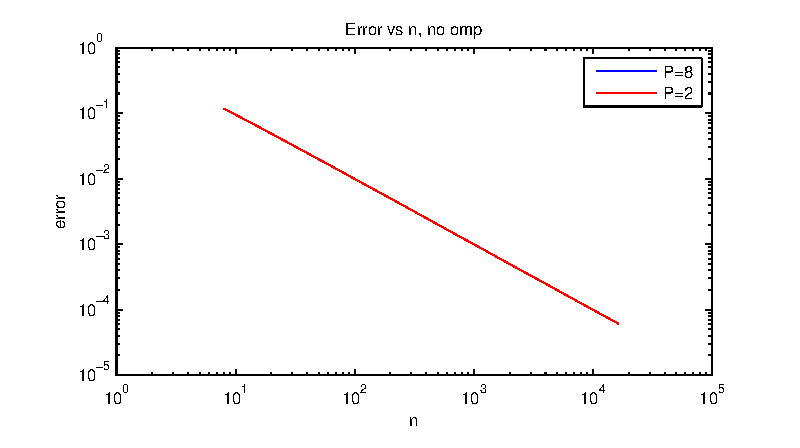
\includegraphics[]{graphics/error.eps}
  \caption{A plot of the error. The two lines overlap perfectly.}
  \label{fig:error}
\end{figure}
% section comparison_of_error_for_p_8_and_p_2 (end)


\section{Memory requirement} % (fold)
\label{sec:memory_requirement}
For the root process (rank 0) the memory requirement $M_0$ is
\begin{equation}
  M_0 = 8 \, \mathrm{bytes} \times n
\end{equation}
where $n$ is the number of elements to be summed. For all other processes, the memory requirement $M_p$ per processor scales with the number of elements $n$ and the number of processors $P$ as follows:
\begin{equation}
  M_p = \frac{8 \, \mathrm{bytes} \times n}{P-1}
\end{equation}

\begin{table}[H]
  \centering
  \caption{The memory required for various numbers of processors and data set sizes. For $P>1$, the memory used by the root process is ignored (it is what's shown in the first row).}
  \label{tab:memoryreq}
  \begin{tabularx}{1.0\textwidth}{X|XXXXXX}
    \toprule
    $n$/$P$  & 8  & 32  & 128  & 1024 & 4096  & 16384 \\
    \midrule
    1        & 64 & 256 & 1024 & 8192 & 32768 & 131072 \\
    2        & 64 & 256 & 1024 & 8192 & 32768 & 131072 \\
    4        & 22 & 86  & 342  & 2731 & 10123 & 43691  \\
    8        & 10 & 37  & 147  & 1171 & 4682  & 18725  \\
    \bottomrule
  \end{tabularx}
\end{table}

% section memory_requirement (end)


\begin{figure}[htbp]
  \centering
  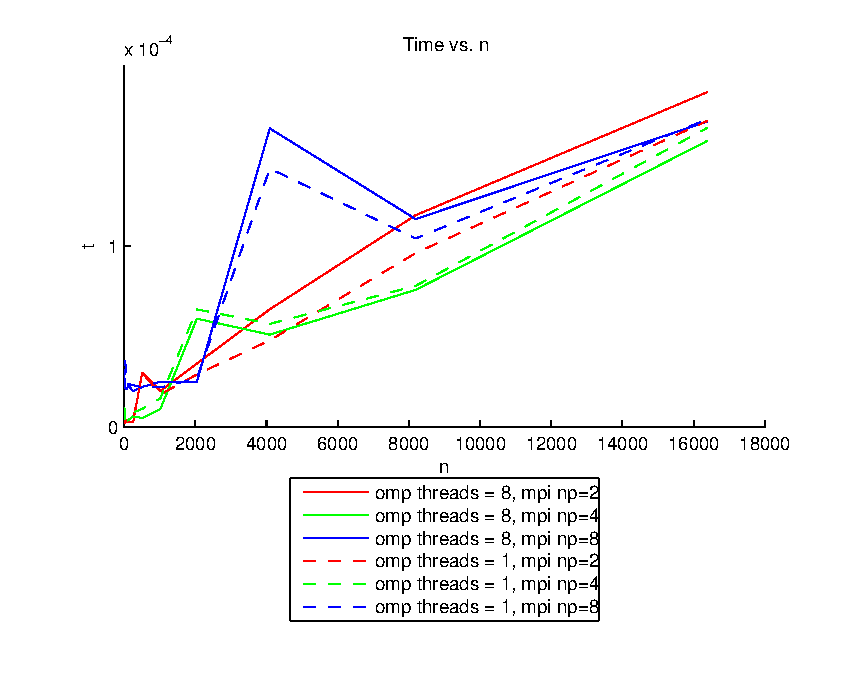
\includegraphics[]{graphics/runtime.eps}
  \caption{A plot of the runtimes for various numbers of processors and data set sizes.}
  \label{fig:runtime}
\end{figure}

\end{document}
